\chapter{Verbs, Tense, and Aspect}\is{verb, verb phrase (VP)|(}

\epigraph{Time's aspects bend, like light through water,\\\phantom{~}\hfill into dappled meanings}{}

If you've ever tried to explain to someone why we say \textit{I'm going to the store} instead of \textit{I go to the store}, or why \textit{I've lived here for five years} means something different from \textit{I lived here for five years}, you've grappled with the complexities of verbs, tense, and aspect.

In this chapter, we'll turn to the world of English verbs, exploring their syntax and semantics, along with the systems of tense and aspect that are so associated with them. We'll start by looking at the two basic verb types: lexical and auxiliary verbs\is{auxiliary verb|(}. We'll set out the special characteristics of the auxiliary verbs (the NICER properties and then consider the morphology~-- the different forms verbs take.

We'll also tackle the issue of tense (distinguishing between grammatical tense and semantic time\is{time!semantic concept vs grammatical tense}), aspect, and modality.

Finally, we'll deal with the issue of verb-phrase complementation~-- the various ways verbs combine with other elements to form complete VPs.

\section{Basic Verb Types}\label{sec:basic-verb-types}\is{modal auxiliary verb|(}\is{lexical verb!vs auxiliary|(}

\begin{figure}[ht]
    \centering
    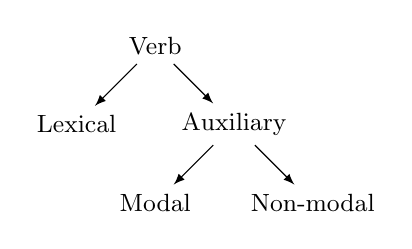
\begin{tikzpicture}[level distance=1cm,
                        sibling distance=2cm,
                        edge from parent/.style={draw, -latex},
                        every node/.style={font=\small, align=center}]

        % Root node
        \node {Verb}
            % First level of branching
            child {node {Lexical}}
            child {node {Auxiliary}
                % Second level of branching
                child {node {Modal}}
                child {node {Non-modal}}
            };

    \end{tikzpicture}
    \caption{Syntactic subclasses of verb}
    \label{fig:verb-structure}
\end{figure}

\noindent When we talk about verbs in English, we're dealing with two main types: lexical verbs and auxiliary verbs. Understanding the difference between them is helpful for grasping how English constructs clauses\is{clause} and conveys certain types of meaning~-- especially since this distinction is far more significant in English than in many other languages\is{cross-linguistic comparison}, such as Spanish\il{Spanish} or Japanese\il{Japanese}, and because auxiliary verbs are involved in a large number of grammatical constructions (e.g., question formation\is{inversion!subject--auxiliary}\is{subject--auxiliary inversion} \& negation\is{negation!and auxiliaries|(}).

\textsc{Lexical verbs} make up the vast majority of different English verbs. With a conservative estimate of around 10,000 verbs in English, over 99\% are lexical. These words express actions (\textit{run},\textit{ eat},\textit{ write}), states\is{stative (verb, etc.)} (\textit{exist},\textit{ seem},\textit{ like}), changes (\textit{become},\textit{ grow},\textit{ turn}), and many other situations. In the sentence \textit{The cat sleeps on the couch}, \textit{sleeps} is the lexical verb, even though not much action is going on.

While lexical verbs carry the weight of meaning, \textsc{auxiliary verbs} often bear the burden of grammar. They help form negatives. They help express aspect\is{aspect|(}. They help construct questions and passive voice\is{passive!be-passive@\textit{be}-passive}
. No wonder they are often called ``helping verbs''. There are very few, but they are in heavy rotation, making up about 36\% of all verbs in a typical English text.

The auxiliary verbs can be further subdivided into: modal and non-modal auxiliaries. \textsc{Modal auxiliaries} express modality~-- notions like possibility, necessity, or obligation\is{modality}. The primary modal auxiliaries in English are \textit{will},\textit{ would},\textit{ can},\textit{ could},\textit{ may},\textit{ might},\textit{ shall},\textit{ should}, and \textit{must}. (See Table~\ref{tab:modal-auxiliary-forms} for their tensed forms.) For example, in \textit{I should study more}, \textit{should} is the modal auxiliary expressing obligation, while \textit{study} is the lexical verb.

Each individual modal auxiliary verb typically has a variety of modal meanings: \textit{can}, for instance, is often associated with ability\is{ability (modality)}, but it also expresses other meanings, as shown in (\ref{ex:can-meanings}).

\ea \label{ex:can-meanings}
\ea \textit{She \uline{can} speak three languages.} \hfill(ability)
\ex \textit{You \uline{can} leave early today.} \hfill(permission)
\ex \textit{It \uline{can} be quite cold here in winter.} \hfill(possibility)
\ex \textit{That \uline{can't} be true!} \hfill(logical conclusion)
\z\z

\noindent And though \textit{should} usually expresses obligation, it occasionally substitutes for conditional \textit{if} as in \textit{Should I be late, please go on without me.}\is{preposition, preposition phrase (PP)!if (conditional)@\textit{if} (conditional)}

The primary non-modal auxiliaries are \textit{be}, \textit{have}, and \textit{do}.

\begin{itemize}[nosep]
    \item \textit{Be} is used to form the progressive aspect\is{progressive aspect} (\textit{I \uline{am} studying}) and passive voice (\textit{The book \uline{was} written}).
    \item \textit{Have} forms the perfect aspect\is{aspect!perfect} (\textit{I \uline{have} studied}).
    \item \textit{Do}\is{do-support@\textit{do}-support|(}\is{auxiliary do@auxiliary \textit{do}|(} is used for emphasis (\textit{I \uline{do} like it}) and in questions (\textit{\uline{Do} you like it?}) and negatives (\textit{No, I \uline{don't} like it}).
\end{itemize}

Few languages rely on auxiliary verbs to the extent that English does. This means that learners from many backgrounds may need extra support to grasp the importance of auxiliaries in forming questions, negatives, and expressing modal meaning in English.

The difference between auxiliaries and lexical verbs becomes clearer when we examine the NICER properties that set auxiliary verbs apart.

\section{The NICER Properties of Auxiliary Verbs}\label{sec:NICER}\is{auxiliary verb!NICER properties|(}

As mentioned in Section \ref{sec:aux}, auxiliary verbs in English have some special properties that set them apart from lexical verbs. These properties are sometimes referred to as the NICER properties, an acronym that stands for Negation\is{negation!and auxiliaries}, Inversion\is{inversion!subject--auxiliary}\is{subject--auxiliary inversion}, Contraction\is{contraction}, Ellipsis\is{ellipsis!VP ellipsis}, and Rebuttal. Let's look at each of these in turn.


\begin{table}[ht]
    \centering
    \renewcommand{\arraystretch}{1.5} % Increase general row height
    \begin{tabular}{>{\raggedright\arraybackslash}m{2cm}>{\raggedright\arraybackslash}m{4.5cm}>{\raggedright\arraybackslash}m{4.5cm}}
       
        \textbf{Property} & \textbf{Auxiliary Verb} & \textbf{Lexical Verb} \\
        \textbf{N}egation & \vspace{4pt}\textit{Lee will not eat apples.}\vspace{4pt} & \vspace{4pt}*\textit{Lee eats not apples.}\vspace{4pt} \\
        \textbf{I}nversion & \vspace{4pt}\textit{Has Lee eaten apples?}\vspace{4pt} & \vspace{4pt}*\textit{Eats Lee apples?}\vspace{4pt} \\
        ``\textbf{C}ontraction'' & \vspace{4pt}\textit{didn't, shouldn't, isn't}\vspace{4pt} & \vspace{4pt}*\textit{eatn't, gon't, maken't}\vspace{4pt} \\
        \textbf{E}llipsis & \vspace{4pt}\textit{Lee was eating and so was Kim.}\vspace{4pt} & \vspace{4pt}*\textit{Lee kept eating and so kept Kim.}\vspace{4pt} \\
        \textbf{R}ebuttal\is{rebuttal} & 
        \vspace{4pt}\parbox[tl]{4.5cm}{
            A: \textit{We shouldn't eat apples.} \\[0.3cm] 
            B: \textit{We should SO.}
        }\vspace{4pt} & 
        \vspace{4pt}\parbox[tl]{4.5cm}{
            A: \textit{We didn't try to eat apples.} \\[0.3cm] 
            B: *\textit{We tried SO.}
        }\vspace{4pt} \\
    \end{tabular}
    \caption{The NICER properties of auxiliary verbs.}
    \label{tab:nicer-properties}
\end{table}
\is{lexical verb!vs auxiliary|)}

Negation in English is typically formed by adding \textit{not} after an auxiliary verb. Lexical verbs, on the other hand, require the auxiliary \textit{do} to form negatives\is{negation!with \textit{do}}. This is called \textsc{do-support@\textit{do}-support}:

\ea
\ea \textit{Lee will not eat apples.}
\ex *\textit{Lee eats not apples.}\footnote{This would have been fine even as recently as Early Modern English\il{English!Early Modern} (the language of Shakespeare), but not today.}
\ex \textit{Lee does not eat apples.}
\z\z

Inversion describes constructions where the auxiliary verb comes before the subject\is{subject (Subj)!and auxiliaries}, such as certain types of questions\is{clause!type and inversion}. Again, lexical verbs need \textit{do} for this:

\protectedex{
\ea
\ea \textit{Has Lee eaten apples?}
\ex *\textit{Eats Lee apples?}
\ex \textit{Does Lee eat apples?}
\z\z}

Inversion for question formation is not a feature shared by a wide range of languages. English learners commonly omit \textit{do} in negation and inversion, likely because it contributes only syntactically, not semantically. For example, they might say \textit{I not like apples} or \textit{He eat apples?} without \textit{do}-support.

``Contraction'' allows \textit{not} to be shortened to -\textit{n't}\is{modal auxiliary verb!negative form} and suffixed to most auxiliary verbs.\footnote{The scare quotes are because there's a difference between a true contraction, like \textit{'s} for \textit{is}, which can go basically anywhere \textit{is} can go and -\textit{n't}, which is a true suffix (see Chapter\ref{ch:vocabulary}}). This isn't possible with lexical verbs:

\ea \textit{didn't}, \textit{shouldn't}, \textit{isn't}
\ex *\textit{eatn't}, *\textit{gon't}, *\textit{maken't}
\z

Ellipsis permits a verb phrase to be understood from the context instead of appearing overtly:

\ea \textit{Lee was eating apples, and Kim was {\op}eating them{\cp} too.}
\ex *\textit{Lee kept eating apples, and Kim kept {\op}eating them{\cp} too.}
\z

Rebuttal\is{rebuttal} uses auxiliary verbs along with \textit{so}, \textit{too}, or \textit{indeed}, to contradict a previous negative statement:

\ea A: \textit{We shouldn't eat apples.}\\
B: \textit{We should SO.}
\ex A: \textit{We didn't try to eat apples.}
\\ B: *\textit{We tried SO.}
\z

The NICER properties are not just helpful diagnostics, they actually identify many of the things about auxiliary verbs that make them challenging for our students. For example, it explains why we say \textit{Don't you like it?} instead of *\textit{You no like it?}, or why you might utter the assertion \textit{I do like it}.\is{negation!and auxiliaries|)}\is{do-support@\textit{do}-support|)}\is{auxiliary do@auxiliary \textit{do}|)}

In the next section, we'll look at the various forms that verbs can take in English, which will set us up to discuss tense and aspect.

\begin{tcolorbox}[title=Exercise: Basic Verb Types, colback=white, colframe=blue!75!black, fonttitle=\bfseries]
Identify whether the underlined verbs in the following sentences are lexical or auxiliary. If auxiliary, specify whether they are modal or non-modal. Remember that some auxiliary verbs have a matching lexical verb.

\begin{enumerate}[nosep]
    \item \textit{The cat \uline{sleeps} on the couch.}
    \item \textit{I \uline{will} attend the meeting tomorrow.}
    \item \textit{She \uline{has} a test tomorrow.}
    \item \textit{She \uline{has} finished her homework.}
    \item \textit{\uline{Did} she \uline{do} her homework?}
    \item \textit{They \uline{are} planning a surprise party.}
    \item \textit{It'\uline{s} at my house.}
    \item \textit{It \uline{is} not.}
    \item \textit{You \uline{must} complete the assignment by Friday.}
    \item \textit{I don't think I \uline{can}.}
\end{enumerate}
For each of the following sentences, apply one of the NICER properties (Negation, Inversion, Contraction, Ellipsis, or Rebuttal) to create a new, grammatically correct sentence. Identify which property you used.

\begin{enumerate}[nosep]
    \item \textit{She can swim very well.}
    \item \textit{They have finished the project.}
    \item \textit{We are having lunch.}
    \item \textit{You should try it.}
    \item \textit{Do you study grammar?}
\end{enumerate}

Example: \textit{He's Cambodian.} $\rightarrow$ \textit{He isn't Cambodian.} (Contraction)
\end{tcolorbox}
\is{NICER properties|)}\is{auxiliary verb!NICER properties|)}

\section{Verb Forms}\label{sec:verb-forms}

English verbs, whether lexical or auxiliary, have several different forms. As a proficient English speaker, you already know their syntax, morphology, and spelling, but, as an English teacher, being able to identify them is useful for understanding and explaining clause structure and the English tense and aspect system.

The \textsc{plain form}\is{plain form of verb} is the simplest form of the verb. It's the ``dictionary form''.

\ea \textit{arrive}, \textit{be}, \textit{come}, \textit{do}, \textit{eat}, \textit{fall}, \textit{go}, \textit{have}, \textit{interrupt}
\z

\begin{table}[ht]
    \centering
    \begin{tabular}{ccccccc}
       
        \textbf{Plain} & \multicolumn{3}{c}{\textbf{Tensed}} & \multicolumn{2}{c}{\textbf{Participles}} \\
        & \multicolumn{2}{c}{\textbf{Present}} & \textbf{Past} & \textbf{Present} & \textbf{Past} \\
        & plain & 3rd pers sing & &  &  \\
        \textit{jump} & \textit{jump} & \textit{jumps} & \textit{jumped} & \textit{jumping} & \textit{jumped} \\
        \textit{go} & \textit{go} & \textit{goes} & \textit{went} & \textit{going} & \textit{gone} \\
        \textit{eat} & \textit{eat} & \textit{eats} & \textit{ate} & \textit{eating} & \textit{eaten} \\
        \textit{put} & \textit{put} & \textit{puts} & \textit{put} & \textit{putting} & \textit{put} \\
        \textit{keep} & \textit{keep} & \textit{keeps} & \textit{kept} & \textit{keeping} & \textit{kept} \\
    \end{tabular}
    \caption{Verb Forms: Plain, Tensed, and Participles}
    \label{tab:verb-forms}
\end{table}

The \textsc{plain present form}\is{present tense}\is{tense!present} is identical to the plain form for all verbs (see Table \ref{tab:verb-forms}) except \textit{be}, which has an unusual number of present forms: \textit{am}, \textit{is}, and \textit{are}.

\ea \textit{arrive}, \textit{come}, \textit{do}, \textit{eat}, \textit{fall}, \textit{go}, \textit{have}, \textit{interrupt}
\z
The \textit{-s} form\is{s form@-\textit{s} verb form}, or the \textsc{third-person singular present form}\is{third-person singular present form}, adds \textit{-{\op}e{\cp}s} to the plain form, with a few irregular forms, as in (\ref{ex:3sing-pres}).

\ea \textit{arrives}, \textit{is}, \textit{comes}, \textit{does}, \textit{eats}, \textit{falls}, \textit{goes}, \textit{has}, \textit{interrupts}\label{ex:3sing-pres}
\z
The \textsc{past form}\is{past tense}\is{tense!past} is used for the simple past tense. Regular verbs add \textit{-ed}, but many common verbs have irregular past forms:

\ea \textit{arrived}, \textit{was}/\textit{were}, \textit{came}, \textit{did}, \textit{ate}, \textit{fell}, \textit{went}, \textit{had}, \textit{interrupted}\label{ex:past-tense-forms}
\z
The \textit{-ing} form\is{ing form@-\textit{ing} verb form}, also known as the \textsc{present participle}\is{participle!present}\label{sec:participles},\footnote{CGEL uses the term \textsc{gerund-participle}\is{gerund-participial (verb-form)} for this form.} is used to form the progressive aspect, among other things:

\ea \textit{arriving}, \textit{being}, \textit{coming}, \textit{doing}, \textit{eating}, \textit{falling}, \textit{going}, \textit{having}, \textit{interrupting}\label{ex:-ing}
\z

\begin{tcolorbox}[title=What about gerunds?\is{gerund@``gerund''}, colback=white]

You may have heard about \textsc{gerunds}~-- verbs in the \textit{-ing} form that ``function as nouns''~-- as in the underlined phrases in (\ref{ex:merely-looking} \& \ref{ex:making-dinner}).

\ea\textit{\uline{Merely looking} can make a difference.}\label{ex:merely-looking}
\ex\textit{I actually enjoy \uline{making dinner} after a long day,} \label{ex:making-dinner}
\z

~~~~The problem is that the idea of a verb functioning as a noun is as odd that of a goldfish functioning as a dog; while both species may function as pets, their fundamental natures remain distinct. Similarly, \textsc{subject}\is{subject (Subj)} and \textsc{complement}\is{complement, complementation!in clause/VP} are functions, but \textsc{noun} is what a word intrinsically is. So, are \textit{looking} and \textit{making} fundamentally nouns or verbs?

~~~~In considering this question, you should return to the characteristics of nouns and verbs you encountered in Sections \ref{sec:nouns} and \ref{sec:verbs}. If the underlined phrases in (\ref{ex:merely-looking} \& \ref{ex:making-dinner}) were NPs, then we might expect them to allow plural forms and AdjP modifiers. They don't. Instead, they allow AdvP\is{adverb, adverb phrase (AdvP)} modifiers\is{modification, modifier} as in \textit{merely looking} and license objects\is{object (Obj)!direct} as in \textit{making dinner}. These are the characteristics of VPs.

~~~~That's not to say that there aren't \textit{-ing} nouns, but they're not so common. They show up in examples like  (\ref{ex:the-opening} \& \ref{ex:building-of}).

\ea    \textit{The \uline{opening} of the new store attracted a large crowd.} \label{ex:the-opening}
\ex   \textit{The city funded the \uline{building} of the bridge.}\label{ex:building-of}
\z

In such cases, the \textit{-ing} words are true nouns:

\begin{itemize}[nosep]
    \item They can be pluralized: \\\textit{The \uline{openings} of the new stores were scheduled for next month.}
    \item They can be modified by adjectives: \\\textit{The \uline{grand opening} of the new store was a success.}
    \item They require a preposition phrase with \textit{of} to introduce their complement: \textit{The building \uline{of} the bridge}, not *\textit{The building the bridge}.
\end{itemize}

These characteristics align with what we expect of nouns.

~~~~So what to do with the term ``gerund''. Personally, I don't find it useful for discussing the English of today. Instead, I would simply say that the subject of  (\ref{ex:merely-looking}) is a VP, as is the complement of \textit{enjoy} in (\ref{ex:making-dinner}).\footnote{\textit{CGEL} would call these clauses, not VPs.}

\end{tcolorbox}

The \textsc{past participle}\is{participle!past} has various grammatical roles, including forming the perfect aspect and passive constructions. For regular verbs, it's identical to the past form (sometimes called the preterite), but many irregular verbs have distinct past participles:

\ea \textit{arrived}, \textit{been}, \textit{come}, \textit{done}, \textit{eaten}, \textit{fallen}, \textit{gone}, \textit{had}, \textit{interrupted}\label{ex:past-participles}
\z

Most lexical verbs\is{lexical verb!vs auxiliary} have all six of these forms, but modal auxiliaries are \textsc{defective}\is{defective verb}\is{modal auxiliary verb!defectiveness}~-- they lack the plain form and participles.\label{sec:defective-modals}

\ea \textit{can}/\textit{could}, \textit{will}/\textit{would}, \textit{shall}/\textit{should}, \textit{may}/\textit{might}, \textit{must}/--
\z

\noindent The auxiliary verbs, modal or not, also have negative and contracted forms.\is{tense|(}\is{modal auxiliary verb!contracted form}\is{modal auxiliary verb!negative form}\is{modal auxiliary verb!present-tense form}\is{modal auxiliary verb!past-tense form}

\begin{table}[ht]
    \centering
    \begin{tabular}{cccccc}
       
        \multicolumn{3}{c}{\textbf{Present Tense}} & \multicolumn{3}{c}{\textbf{Past Tense}} \\
         & Contracted & Negative &  & Contr. & Negative \\
        \textit{will} & \textit{'ll} & \textit{won't} & \textit{would} & \textit{'d} & \textit{wouldn't} \\ 
        \textit{may} & & & \textit{might} & & \textit{mightn't} \\ 
        \textit{can} & & \textit{can't}, \textit{cannot} & \textit{could} & & \textit{couldn't} \\ 
        \textit{shall} & \textit{'ll} & \textit{shan't} & \textit{should} & & \textit{shouldn't} \\ 
        \textit{must} & & \textit{mustn't} & & & \\
        \textit{do} & \textit{do}(\textit{es})\textit{n't} & & \textit{did} & \textit{didn't} & \\ 
        \textit{have} & \textit{'ve}/\textit{'s} & \textit{haven't}/\textit{hasn't} & \textit{had} & \textit{'d} & \textit{hadn't} \\ 
        \textit{be} & \textit{'m}/\textit{'re}/\textit{'s} & \textit{--}/\textit{aren't}/\textit{isn't} & \textit{was}/\textit{were} & & \textit{wasn't}/\textit{weren't} \\
    \end{tabular}
    \caption{Tensed auxiliary verb forms}
    \label{tab:modal-auxiliary-forms}
\end{table}
\is{modal auxiliary verb|)}

\noindent The non-modal auxiliaries~-- \textit{do}, \textit{have}, and \textit{be}~-- also have plain, present-participle, and past participle forms. It's also worth noting that these three verbs also have lexical-verb counterparts. In each case, we know they're not modal because the NICER properties don't apply.

\ea
\ea \textit{Don't \uline{be} late.}\label{ex:lexical-be}
\ex \textit{I \uline{have} a cat.}\label{ex:lexical-have}
\ex \textit{I \uline{do} my homework every day.}\label{ex:lexical-do}
\z\z
In (\ref{ex:lexical-be}), we can't have *\textit{Be not late} or even *\textit{ben't}. In (\ref{ex:lexical-have}), we have the verb of belonging, not the one that forms the perfect aspect. We don't ask \textit{Have you a cat?} or say \textit{I haven't a cat} (at least not in most present-day North American dialects). And if we want to ask about doing your homework, we need an auxiliary \textit{do} (underlined) to go with the lexical \textit{do}: \textit{\uline{Do} you do your homework?}

The verb \textit{be} is highly irregular, with more forms than any other English verb:

\ea
\ea \textit{be}, \textit{am}, \textit{is}, \textit{are}, \textit{was}, \textit{were}, \textit{being}, \textit{been}
\ex \textit{isn't}, \textit{aren't}, \textit{wasn't}, \textit{weren't}
\ex \textit{'m}, \textit{'s}, \textit{'re}
\z\z

The various verb forms combine with auxiliaries to create the tense and aspect system. For instance, the present perfect\is{present perfect} uses \textit{have} + the past-participle form:\footnote{In \cite{Huddleston2002}, the perfect is a secondary past tense, but I don't find that analysis helpful here, and so I don't follow it.}

\ea \textit{I have eaten.}
\ex \textit{She has gone.}
\z

The past progressive combines the past of \textit{be} with the \textit{-ing} form:

\ea \textit{I was reading.}
\ex \textit{They were sleeping.}
\z\is{progressive aspect}\is{aspect!perfect}

\begin{tcolorbox}[title=Exercise: Verb Forms, colback=white, colframe=red!75!black, fonttitle=\bfseries]
Identify the verb form (1. plain, 2. plain present, 3. third-person singular present, 4. past, 5. present participle, or 6. past participle) for each underlined verb.

\begin{enumerate}[nosep]
    \item \textit{She \uline{sings} beautifully.} \hfill\uline{~~~~}
    \item \textit{They \uline{may} \uline{have} \uline{gone} to the store.} \hfill\uline{~~~~},  \uline{~~~~},  \uline{~~~~}
    \item \textit{We \uline{were} \uline{watching} a movie.} \hfill\uline{~~~~},  \uline{~~~~}
    \item \textit{The dog \uline{barked} all night.} \hfill\uline{~~~~}
    \item \textit{I \uline{write} in my journal every day.} \hfill\uline{~~~~}
    \item \textit{I'\uline{ll} \uline{try} again.} \hfill\uline{~~~~},  \uline{~~~~}
\end{enumerate}
\end{tcolorbox}
\is{auxiliary verb|)}\is{complement, complementation|)}\is{tense|)}\is{aspect|)}

\section{Aspect}\is{aspect|(}
If tense is primarily about when something happens, \textsc{aspect} is more about the temporal perspective we take on a situation. But what does that really mean?

\subsection{The progressive aspect}\is{progressive aspect|(}\label{sec:progressive-aspect}
Let's start with a seemingly simple question: what's the difference between these two sentences?

\ea
\ea \textit{I live in Mississauga.} \hfill(simple aspect) \label{ex:I-live}
\ex \textit{I'm living in Mississauga.} \hfill(progressive aspect) \label{ex:Im-living}
\z\z

At first glance, these sentences might appear identical~-- both state my city of residence and both are factually correct. But there's a subtle distinction: (\ref{ex:I-live}) suggests an indifference to the duration of the situation, while (\ref{ex:Im-living}) asserts the relevance of its temporariness. This difference in perspective is illustrated in Figure~\ref{fig:enter-label}.

\begin{figure}[ht]
    \centering
    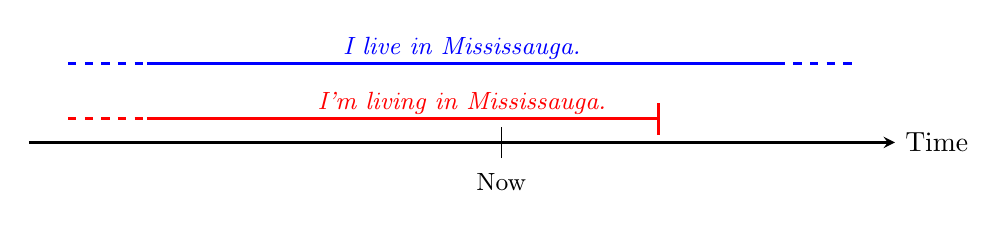
\begin{tikzpicture}[scale=1]
        % Define styles
        \tikzset{
            timeline/.style={->, >=stealth, thick},
            label/.style={font=\small}
        }
        % Draw the main timeline
        \draw[timeline] (-1,0) -- (10,0) node[right] {Time};
        % "Now" point on timeline
        \draw (5,-0.2) -- (5,0.2);
        \node[label] at (5,-0.5) {Now};
        % "I live in Mississauga" (Simple aspect)
        \draw[blue, very thick, dashed] (-0.5,1) -- (0.5,1);
        \draw[blue, very thick] (0.5,1) -- (8.5,1);
        \draw[blue, very thick, dashed] (8.5,1) -- (9.5,1);
        \node[label, blue] at (4.5,1.2) {\textit{I live in Mississauga.}};
        % "I'm living in Mississauga" (Progressive aspect)
        \draw[red, very thick, dashed] (-0.5,0.3) -- (0.5,0.3);
        \draw[red, very thick] (0.5,0.3) -- (7,0.3);
        \node[label, red] at (4.5,0.5) {\textit{I'm living in Mississauga.}};
        \draw[red, very thick] (7,0.5) -- (7,0.1);  % End vertical bar
    \end{tikzpicture}
    \caption{Comparison of the simple and progressive aspects for \textit{I live in Mississauga} on a timeline.}
    \label{fig:enter-label}
\end{figure}

Anyone might say (\ref{ex:I-live}) in the simple aspect, but only someone like an international student attending University of Toronto would choose the progressive aspect of (\ref{ex:Im-living}). While all situations are ultimately ephemeral, the progressive aspect, formed with $be+-ing$ expresses relevance not just to what continues but to its conclusion. The simple aspect, in contrast, draws no special attention to endings.

To illustrate this shift in viewpoint, consider the difference between paddling a river that flows into the sea vs paddling one that comes to a dam. It's the same body of water either way, but in the first, you're aware only of the water, while in the second, the dam requires your attention.

Unlike these paddlers, a speaker typically has a choice of how to portray the situation. The selection of one aspect or the other invites the audience to consider the situation from a particular vantage point, with neither being grammatically better.

\subsubsection{States often resist the progressive aspect}\label{sec:statives-resist}
Sometimes, though, one perspective really does seem wrong to certain groups of speakers. Consider, for instance, (\ref{ex:know-knowing}).

\ea \label{ex:know-knowing}
\ea \textit{I know that feeling.}
\ex *\textit{I'm knowing that feeling.}
\z\z

The progressive in (\ref{ex:know-knowing}b) implies that an endpoint to this knowledge is relevant, a perspective that feels unnatural. For many speakers of English, drawing attention to the potential cessation of knowing is odd, not because knowledge can't end~-- people do forget~-- but because it's so clearly not relevant. The simple aspect, by contrast, allows us to focus on the current state of knowing without unnecessary implications about its duration.\footnote{\ref{ex:know-knowing}b is, nevertheless, quite common in South Asian English\il{English!South Asian}, for example.}

The same applies to other verbs. Consider the stative\is{stative (verb, etc.)|(} examples in (\ref{ex:stative-verbs}). The (a) sentences with the simple aspect are fine, but the (b) examples in the progressive are ungrammatical.

\ea\label{ex:stative-verbs}
\ea \textnormal{i.} \textit{Birds have feathers.} \\ \textnormal{ii.} \textit{Earth is a planet.} \\ \textnormal{iii.} \textit{Honey tastes sweet.}
\ex \textnormal{i.} *\textit{Birds are having feathers.} \\ \textnormal{ii.} *\textit{Earth is being a planet.} \\ \textnormal{iii.} *\textit{Honey's tasting sweet.}
\z\z

The end of birds having feathers, of Earth being a planet, or of honey tasting sweet might be relevant in some peculiar context, but it's scarcely conceivable what that context might be. By asking us to take an irrelevant perspective with these \textsc{stative verbs}, the progressive aspect creates a linguistic mismatch and registers as ungrammatical.

And yet, sometimes it works, as in (\ref{ex:prog-statives}).

\ea\label{ex:prog-statives}
\ea \textit{We're having dinner.}
\ex \textit{He's being grumpy.}
\ex \textit{It's tasting sweeter.}
\z\z

In these cases, the progressive aspect fits because the impending end of the state matters. I can call you back when the meal is over, it would be better to talk to him when he's no longer grumpy, and presumably, the honey will soon return to its usual taste once the effect of whatever changed it has worn off. These examples demonstrate that the progressive aspect isn't inherently ungrammatical with stative verbs. It's just not usually a good fit.\is{stative (verb, etc.)|)}

\subsubsection{Progressive aspect for limited repetition}\is{progressive aspect|(}
While most actions take time, others are instantaneous: \textit{the light flashed, she sneezed, it popped, he blinked, the show ended}. In cases like these, the progressive aspect can still be used. But rather than inviting us to consider the end of a single situation, it asserts the relevance of the end of a series of events. \textit{I'm falling} may be a long drawn out descent, but \textit{She's sneezing} doesn't imply a super slow-mo spit-spraying expulsion of air. Instead it presents a set of sternutations for which an end is in sight.

This interpretation of the progressive aspect as indicating a limited series isn't restricted to momentary events. \textit{I'm going to the gym regularly} is the claim of a person who's not sure how long they can keep up the commitment or has a limited-term membership, as in Figure~\ref{fig:regular-gym-visits}.

\begin{figure}[ht]
    \centering
    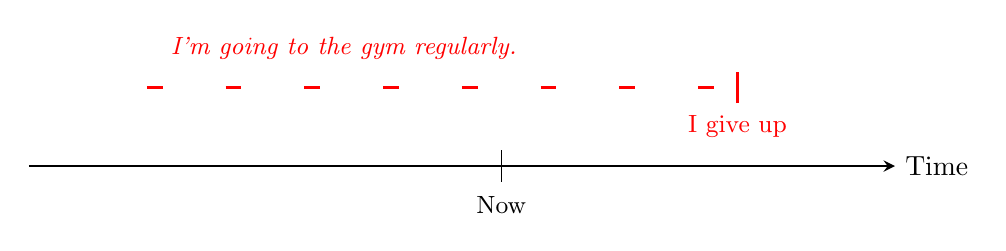
\begin{tikzpicture}[scale=1]
        % Define styles
        \tikzset{
            timeline/.style={->, >=stealth, thick},
            label/.style={font=\small}
        }
        % Draw the main timeline
        \draw[timeline] (-1,0) -- (10,0) node[right] {Time};
        % "Now" point on timeline
        \draw (5,-0.2) -- (5,0.2);
        \node[label] at (5,-0.5) {Now};
        % "end" point on timeline
        \draw[red, very thick] (8,0.8) -- (8,1.2);
        \node[label, red] at (8,0.5) {I give up};
        % Event instances (e.g., gym visits)
        \foreach \x in {0.5, 1.5, 2.5, 3.5, 4.5, 5.5, 6.5, 7.5}
            \draw[red, very thick] (\x,1) -- (\x+0.2,1);
        % Labels for periodic gym visits
        \node[label, red] at (3, 1.5) {\textit{I'm going to the gym regularly.}};
    \end{tikzpicture}
    \caption{Timeline for the progressive aspect in \textit{I'm going to the gym regularly}.}
    \label{fig:regular-gym-visits}
\end{figure}

Another illustrative example of this phenomenon is \textit{I'm eating at that new restaurant}. While eating a meal is not an instantaneous action, the use of the progressive aspect here doesn't necessarily imply that the speaker is currently in the middle of a meal at the restaurant. Instead, it suggests a series of visits until something new comes along.

In the gym example, the use of \textit{regularly} makes the repeated-temporary-action interpretation the only possible meaning of the progressive. The restaurant example, though, is ambiguous. If said outside the restaurant, then it implies serial patronage. If inside, perhaps it refers to a meal that will end before some other relevant event.

\subsubsection{The progressive for plans}
The progressive aspect has yet more uses. It can also express future plans, as it does in (\ref{ex:dinner-next-week}).

\ea \textit{The Smiths are having dinner with us this week.}\label{ex:dinner-next-week}
\z

This doesn't imply an ongoing, extended feast. Rather, it encapsulates the planning and anticipation of the event. This usage presupposes that the dinner has been arranged; the progressive aspect wouldn't be appropriate if the idea had just occurred and the Smiths hadn't been invited yet. The progressive here spans from the moment of agreement (the start) to the anticipated conclusion of the dinner (the end).
\is{progressive aspect|)}

\begin{figure}[ht]
    \centering
    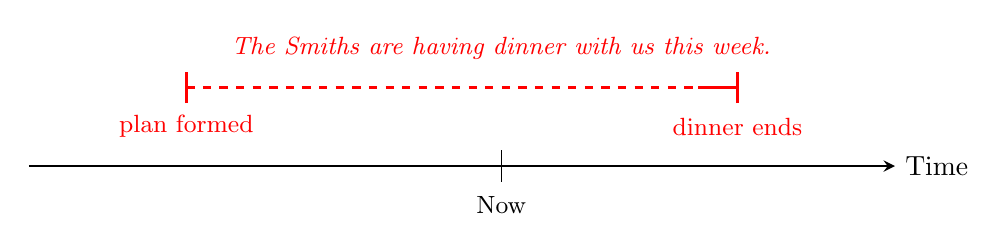
\begin{tikzpicture}[scale=1]
        % Define styles
        \tikzset{
            timeline/.style={->, >=stealth, thick},
            label/.style={font=\small}
        }
        % Draw the main timeline
        \draw[timeline] (-1,0) -- (10,0) node[right] {Time};
        % "Now" point on timeline
        \draw (5,-0.2) -- (5,0.2);
        \node[label] at (5,-0.5) {Now};
        % "We're having dinner with the Smiths next week" (Future Progressive aspect)
        \draw[red, very thick, dashed] (1,1) -- (7.5,1); % Planning phase - from now
        \draw[red, very thick] (7.5,1) -- (8,1); % Future event
        \draw[red, very thick] (1,0.8) -- (1,1.2); % Start boundary of event
        \draw[red, very thick] (8,0.8) -- (8,1.2); % End boundary of event
        \node[label, red] at (5,1.5) {\textit{The Smiths are having dinner with us this week.}};
        % Add "planned" below the planning phase
        \node[label, red] at (1, 0.5) {plan formed};
        % Add "dinner" below the planning phase
        \node[label, red] at (8, 0.5) {dinner ends};
    \end{tikzpicture}
    \caption{Representation of the ``planned future'' use of the progressive aspect for \textit{We're having dinner with the Smiths next week.}}
    \label{fig:futurate-progressive}
\end{figure}
\is{progressive aspect|)}

\subsection{The perfect aspect}\is{aspect!perfect|(}\label{sec:perfect-aspect}
While the progressive aspect focuses on the ongoing nature of a situation, English has another aspect that expresses a different temporal perspective: the perfect. The perfect aspect, formed with a form of have + past participle\is{participle!past|(}, asserts the relevance of a previous situation (or action, etc) to a later time.

The reference time can be in the present, past, or even in the future, but let's start with the present perfect\is{present perfect|(}. This uses the present tense and has "now" as a reference time. Consider (\ref{ex:have-lived}).

\ea \textit{I've lived in Mississauga for five years.}\label{ex:have-lived}
\z

In its most salient sense, this sentence conveys a situation that began in the past and continues to be true in the present. It stretches back for five years and remains relevant now. To appreciate the nuance of the perfect aspect, let's compare it to the simple past\is{past tense}\is{tense!past}:

\ea \textit{I lived in Mississauga for five years.}\label{ex:lived}
\z

In (\ref{ex:lived}), I'm talking about a situation fully in the past. I no longer live there. The cases of the present-perfect (\ref{ex:have-lived}) case and the simple past (\ref{ex:lived}) are contrasted in Figure~\ref{fig:past-vs-present-perfect}. Non "now" reference times are shown in Figures~\ref{fig:past-perfect}--\ref{fig:timeless-perfect}. In each case, the perfect aspect connects two time points: the time of the situation itself and the subsequent reference time to which it's relevant. This allows speakers to express complex temporal relationships and emphasize the significance of past (or completed future) situations to other points in time.

\begin{figure}[ht]
    \centering
    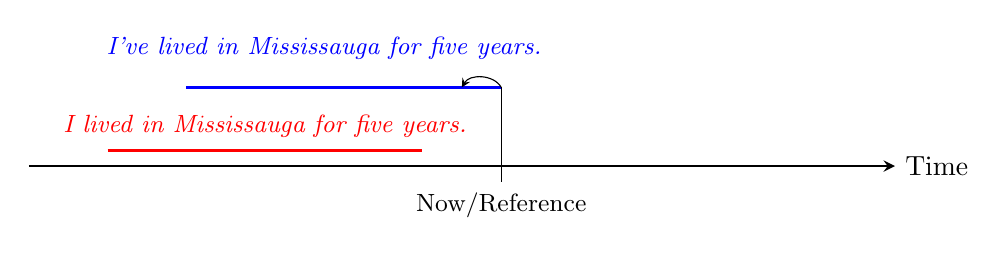
\begin{tikzpicture}[scale=1]
        % Define styles
        \tikzset{
            timeline/.style={->, >=stealth, thick},
            label/.style={font=\small}
        }
        % Draw the main timeline
        \draw[timeline] (-1,0) -- (10,0) node[right] {Time};
        % "Now" point on timeline
        \draw (5,-0.2) -- (5,1);
        \node[label] at (5,-0.5) {Now/Reference};
        % "I've lived in Mississauga for five years" (Present Perfect aspect)
        \draw[blue, very thick] (1,1) -- (5,1); % From past to now
        \node[label, blue] at (2.75,1.5) {\textit{I've lived in Mississauga for five years.}};
        % "I lived in Mississauga for five years" (Simple Past aspect)
        \draw[red, very thick] (0,0.2) -- (4,0.2); % A completed action in the past, same length but before now
        \node[label, red] at (2,0.5) {\textit{I lived in Mississauga for five years.}};
        % Arcing arrow
        \draw[->, >=stealth, bend right=60] (5,1) to (4.5,1);
    \end{tikzpicture}
    \caption{Comparison of the present perfect and simple past for \textit{I lived in Mississauga for five years.} The reference point is ``now''.}
    \label{fig:past-vs-present-perfect}
\end{figure}

\begin{figure}[ht]
    \centering
    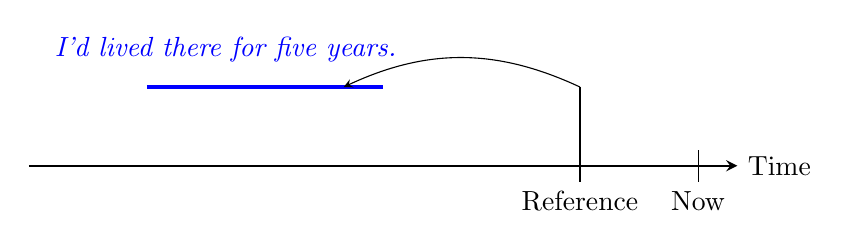
\begin{tikzpicture}
        % Timeline
        \draw[->, >=stealth, thick] (0,0) -- (9,0) node[right] {Time};
        % "Reference" point
        \draw (7,-0.2) -- (7,1);
        \node[below] at (7,-0.2) {Reference};
        % "Now" point
        \draw (8.5,-0.2) -- (8.5,0.2);
        \node[below] at (8.5,-0.2) {Now};
        % Past perfect duration
        \draw[blue, very thick] (1.5,1) -- (4.5,1);
        % Example text
        \node[blue, above] at (2.5,1.2) {\textit{I'd lived there for five years.}};
        % Arcing arrow
        \draw[->, >=stealth, bend right=25] (7,1) to (4,1);
    \end{tikzpicture}
    \caption{Representation of the past perfect: \textit{I'd lived there for five years.} The reference point is before ``now'', and the situation is fully before that point.}
    \label{fig:past-perfect}\is{past perfect}
\end{figure}

\begin{figure}[ht]
    \centering
    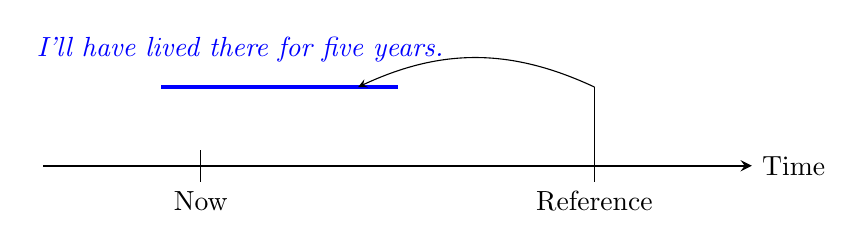
\begin{tikzpicture}
        % Timeline
        \draw[->, >=stealth, thick] (0,0) -- (9,0) node[right] {Time};
        % "Now" point
        \draw (2,-0.2) -- (2,0.2);
        \node[below] at (2,-0.2) {Now};
        % "reference" point
        \draw (7,-0.2) -- (7,1);
        \node[below] at (7,-0.2) {Reference};
        % Futurate perfect duration
        \draw[blue, very thick] (1.5,1) -- (4.5,1);
        % Example text
        \node[blue, above] at (2.5,1.2) {\textit{I'll have lived there for five years.}};
        % Arcing arrow
        \draw[->, >=stealth, bend right=25] (7,1) to (4,1);
    \end{tikzpicture}
    \caption{Representation of the futurate perfect: \textit{I'll have lived there for five years.} The reference point after ``now'' and the event is before that point. Note the ``now'' could be anywhere before the end of the blue line.}
    \label{fig:futurate-perfect}\is{futurate}
\end{figure}

\begin{figure}[ht]
    \centering
    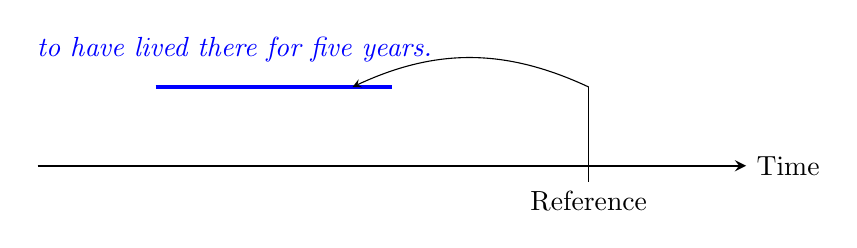
\begin{tikzpicture}
        % Timeline
        \draw[->, >=stealth, thick] (0,0) -- (9,0) node[right] {Time};
        % "reference" point
        \draw (7,-0.2) -- (7,1);
        \node[below] at (7,-0.2) {Reference};
        % Futurate perfect duration
        \draw[blue, very thick] (1.5,1) -- (4.5,1);
        % Example text
        \node[blue, above] at (2.5,1.2) {\textit{to have lived there for five years.}};
        % Arcing arrow
        \draw[->, >=stealth, bend right=25] (7,1) to (4,1);
    \end{tikzpicture}
    \caption{Representation of the timeless perfect: \textit{To have lived there for five years is quite an experience.} The reference point is any time.}
    \label{fig:timeless-perfect}
\end{figure}

The perfect aspect can sometimes lead to ambiguity. The situation must begin prior to the reference time, but whether or not it is complete at the reference time is open to interpretation. As a result, the red line in Figure~\ref{fig:present-perfect-simple-past} representing the simple past and the blue line immediately above it may refer to exactly the same period of time, just from different perspectives. The ambiguity can usually be resolved from the context, or from some modifier such as \textit{already} (completed).

\begin{figure}[ht]
    \centering
    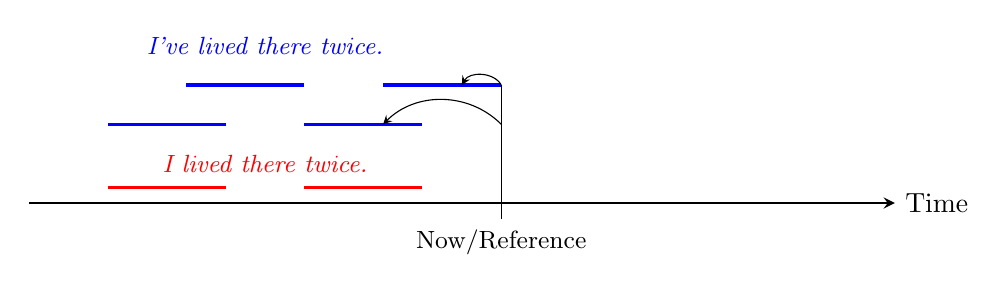
\begin{tikzpicture}[scale=1]
        % Define styles
        \tikzset{
            timeline/.style={->, >=stealth, thick},
            label/.style={font=\small}
        }
        % Draw the main timeline
        \draw[timeline] (-1,0) -- (10,0) node[right] {Time};
        % "Now" point on timeline
        \draw (5,-0.2) -- (5,1.5);
        \node[label] at (5,-0.5) {Now/Reference};
        % "I've lived in Mississauga for five years" (Present Perfect aspect)
        \draw[blue, very thick] (0,1) -- (1.5,1);
        \draw[blue, very thick] (2.5,1) -- (4,1); % From past to now
        % "I've lived in Mississauga for five years" (Present Perfect aspect)
        \draw[blue, very thick] (1,1.5) -- (2.5,1.5);
        \draw[blue, very thick] (3.5,1.5) -- (5,1.5); % From past to now
        \node[label, blue] at (2,2) {\textit{I've lived there twice.}};
        % "I lived in Mississauga for five years" (Simple Past aspect)
        \draw[red, very thick] (0,0.2) -- (1.5,0.2);
        \draw[red, very thick] (2.5,0.2) -- (4,0.2); % A completed action in the past, same length but before now
        \node[label, red] at (2,0.5) {\textit{I lived there twice.}};
        % Arcing arrow
        \draw[->, >=stealth, bend right=45] (5,1) to (3.5,1);
        % Arcing arrow
        \draw[->, >=stealth, bend right=60] (5,1.5) to (4.5,1.5);
    \end{tikzpicture}
    \caption{Comparison of the present perfect and simple past for two periods of residence. The reference point is ``now''.}
    \label{fig:present-perfect-simple-past}
\end{figure}

As you explain these distinctions to your students, you might find yourself grappling with questions like: Why does English need all these different ways of talking about time? How do other languages express these nuances? And how can we help our students not just understand these forms, but feel them intuitively?\is{present perfect|)}\is{aspect!perfect|)}

\begin{tcolorbox}[title=Exercise: Aspect, colback=white, colframe=purple!75!black, fonttitle=\bfseries]
Identify the aspect (simple, progressive, or perfect) in each sentence and explain the temporal perspective it conveys.

\begin{enumerate}[nosep]
    \item \textit{I've worked here for ten years.} \hfill\uline{\hspace{2cm}} tense
    \item \textit{She was reading when the phone rang.} \hfill\uline{\hspace{2cm}} tense~~\uline{\hspace{2cm}} tense
    \item \textit{We play tennis every Saturday.} \hfill\uline{\hspace{2cm}} tense
    \item \textit{They will have completed the course by June.} \hfill\uline{\hspace{2cm}} tense~~\uline{\hspace{2cm}} tense
    \item \textit{The sun is setting earlier these days.}  ~\hfill\uline{\hspace{2cm}} tense
\end{enumerate}
\end{tcolorbox}
\is{participle!past|)}
\is{aspect|)}

\section{Tense Across Languages}\is{cross-linguistic comparison|(}

Imagine for a moment that you're learning a language where verbs don't change to show when something happened. No \textit{-ed} endings for past tense, no \textit{will}. How would you talk about time? It might seem impossible, but for speakers of many languages, this is perfectly normal.

In Mandarin Chinese\il{Chinese!Mandarin}, for instance, the verb form stays the same regardless of when the action occurs:

\ea \textit{Wǒ chī píngguǒ.} (I eat apple)\label{ex:chī}
\z
Example (\ref{ex:chī}) could mean `I eat apples', `I ate an apple', `I'm eating an apple', or `I will eat an apple', depending on the context. Time is often indicated by other words like the equivalent of \textit{tomorrow} or \textit{before}, or it's left to context.

As English speakers, we might find this mind-boggling. But before we get too comfortable with our own tense system, consider the Yimas\il{Yimas} language of Papua New Guinea. It has not two, not three, but seven distinct tenses:\footnote{Some Yimas forms encode both tense and aspect, making them better analyzed as tense--aspect amalgams rather than pure tenses.}

\ea
\ea \textit{wa-ntut} \hfill`went more than a few days ago'
\ex \textit{wa-kiantut} \hfill`went a few days ago'
\ex \textit{wa-nan} \hfill`went yesterday'
\ex \textit{wa-t} \hfill`went today'
\ex \textit{wa-n} \hfill`going now'
\ex \textit{wa-wat} \hfill`usually go'
\ex \textit{wa-kiak} \hfill`will go tomorrow'
\ex \textit{wa-kt} \hfill`will go after tomorrow'
\z\z

These examples highlight a crucial point: the way we conceptualize and express time is not universal. It's just the way each speech community has come to, and speakers of other languages have often arrived at different conventions.

So, given this diversity, how many tenses would you guess English has? Three? Sixteen? In fact, English has \dots

\begin{tcolorbox}[title=Exercise: Comparing Tense and Aspect Across Languages, colback=white, colframe=blue!75!black, fonttitle=\bfseries]

Often the elements that seem very important in one language are simply left out in another. English speakers learning French\il{French} often want to translate the progressive aspect directly, and French has a form for that: \textit{I'm doing it} can be translated as \textit{Je suis en train de le faire.} But even though you \textit{can} translate it like that, usually you wouldn't. You'd just say \textit{je le fais.} French speakers generally just don't care to have their attention brought to the potential end of the event. They don't find it relevant.

~~~~Conversely, some languages regularly mark distinctions that English speakers might not consider. For instance, in Quechua\il{Quechua}, speakers must indicate how they know what they're saying~-- whether they witnessed it themselves, heard it from someone else, or inferred it from evidence. This evidential marking can feel unusual for English speakers, who may not typically specify their information source unless it's directly relevant. In Quechua, however, saying something like \textit{the llama escaped} without indicating the knowledge source (e.g., sight, hearsay, or inference) would be incomplete or even misleading.

Reflect on the following:
\begin{itemize}[nosep]
    \item If you are proficient in another language, consider how it handles aspect. Can it mark the progressive aspect (as English does), for instance? And if it can, does it do so as much as English?
\end{itemize}

\end{tcolorbox}

\section{Tense and Time}\is{cross-linguistic comparison|)}\label{sec:tense-vs-time}\is{time!semantic concept vs grammatical tense|(}

But, first, we need to make a crucial distinction: tense\is{tense!vs time} is not the same as time. Tense is a grammatical category, typically marked on the verb.\footnote{``Typically'' because Japanese\il{Japanese}, for example, has a class of adjectives that conjugate for tense.} Time, on the other hand, is a semantic concept~-- it's about when things happen. It refers to something that physicists are concerned with, something that can be measured.

So, if tense is simply a grammatical category, albeit one that generally has a time-based semantics, how many tenses does English actually have?

Only two: past\is{past tense|(}\is{tense!past|(} and non-past\is{present tense|(}\is{tense!present} (which we usually call ``present tense"). Don't believe me? Let's look at some examples:

\protectedex{
\ea\label{ex:walked-walk to school}
\ea \textit{I \uline{walked} to school yesterday.} \hfill(past tense) 
\ex \textit{I \uline{would} walk to school yesterday.} \hfill(past tense) 
\ex \textit{I \uline{walk} to school every day.} \hfill(present tense)
\ex \textit{I'\uline{m} walking to school right now.} \hfill(present tense)
\ex \textit{I'\uline{m} going to walk to school tomorrow.} \hfill(present tense)
\ex \textit{I'\uline{ll} walk to school tomorrow.} \hfill(present tense)
\z\z}
Notice anything strange? In (\ref{ex:walked-walk to school}c--f) the verbs are all present tense \textit{walk}, \textit{am}, and \textit{will}, even though they're talking about different times. The only past-tense forms are in (a \& b), where we use \textit{walked} and \textit{would}.

``But wait," I hear you say, ``Isn't \textit{I'll walk} in (f) the future tense?" Not quite. \textit{Will} is actually a modal auxiliary verb\is{modal auxiliary verb!tense vs time} in the present tense. It expresses a high degree of certainty about an event, but it's not a tense in itself. It's not even necessarily about future time.

Consider the situation where your friend is coming to visit you. You're busy right now and haven't checked your phone, but the plane was supposed to arrive an hour ago. You have no reason to believe anything different, so, with a high degree of certainty you can say \textit{she'll have landed an hour ago}. Notice that you use \textit{will}, but an hour ago is not the future.

This might seem like a technicality, but it has real implications for how we teach and learn English. For one thing, it explains why English has so many ways of talking about the future\is{futurate|(}:

\ea\label{ex:futurate1} \textit{I\uline{'ll see} you tomorrow.} \hfill(\textit{will} + infinitival)\is{infinitival!clause, VP}
\ex \textit{I\uline{'m seeing} the doctor next week.} \hfill(present progressive)
\ex \textit{My flight \uline{leaves} at 6pm.} \hfill(simple present)
\ex\label{ex:futurate4} \textit{I\uline{'m going to visit} my parents this weekend.} \hfill(\textit{be going to} + infinitival)
\z
Each of (\ref{ex:futurate1}--\ref{ex:futurate4}) is grammatically present tense, but, semantically, they're all talking about future time. There's no single English ``future tense" to learn~-- instead, there's a whole array of present-tense constructions that can refer to future time.\is{futurate|)}

But it's actually not limited to the present tense. Remember how we said tense is about grammar, not meaning? Well, sometimes English uses past tense forms to talk about present or future time:

\ea\label{ex:wish-I-knew} \textit{I wish I \uline{knew} the answer.}\hfill(present time, past tense form)
\ex\label{ex:I-won} \textit{If I \uline{won} the lottery, I'd buy a house.} \hfill(future possibility, past tense form)
\z
In (\ref{ex:wish-I-knew} \& \ref{ex:I-won}), the past tense isn't about time at all~-- it's expressing something about the speaker's perception of likelihood or reality.

As teachers, we often find ourselves grappling with how to explain these subtleties to our students. Do we stick with the familiar but inaccurate ``past, present, future tense" model because it seems logical? Or do we present the simpler yet somewhat less intuitive facts of tense in English?

A general difficulty that this brings up is that we want~-- even expect~-- there to be a one-to-one form-meaning relationship. But we've already seen that the situation is often quite the opposite: it's not only adjective phrases that function as modifiers in NPs; prepositions take a wide range of complements, not just NP objects; and the modal auxiliary verb \textit{can} isn't just for ability\is{ability (modality)}. So too do we find that neither tense is limited to a single meaning. In fact, as we will see later, the time meaning of tense has been almost entirely replaced in the modal auxiliary verbs with other meanings.\is{time!semantic concept vs grammatical tense|)}\is{past tense|)}\is{tense!past|)}\is{present tense|)}\is{tense!present|)}

\begin{tcolorbox}[title=Exercise: Tense and Time, colback=white, colframe=orange!75!black, fonttitle=\bfseries]
For each underlined string, identify the grammatical tense (past or present) and the semantic time (past, present, or future) being expressed. Explain any discrepancies between grammatical tense and semantic time.

\begin{enumerate}[nosep]
    \item \textit{I \uline{wish} I \uline{knew} the answer.}
    \item \textit{The train \uline{leaves} at 5 PM tomorrow.}
    \item \textit{If I \uline{won} the lottery, I \uline{would} buy a house.}
    \item \textit{She \uline{has lived} here for ten years.}
    \item \textit{We \uline{are meeting} the client next week.}
\end{enumerate}

E.g., \textit{I'\uline{m going to visit} my dad this weekend.}  present tense, future time\\
(\textit{Am} is present tense, but the sentence refers to a future visit. It's also about a present plan though.)
\end{tcolorbox}

\section{The English tense/aspect system}\label{sec:tense-aspect}\is{tense!system of|(}\is{aspect!system of|(}

If you've ever tried to create a chart of all the possible English verb forms, you might have ended up with something that looks more like a complex subway map than a neat grammatical table. But it can actually be made quite simple if you are willing to let go of the traditional analysis of ``tenses''.

First, let's recap: we have the past and non-past (present) tenses, along with the simple, perfect, and progressive aspects. If we include the non-tensed infinitival forms\is{infinitival!clause, VP}, the result is Table~\ref{tab:tense-aspect}.

\begin{table}[ht]
    \centering
    \begin{tabular}{ccccc}
        & \textbf{Simple} & \textbf{Progressive} & \textbf{Perfect} & \textbf{Perfect-Progressive} \\
        \textbf{Present} & 
        \textit{I try} & 
        \textit{I am trying} & 
        \textit{I have tried} & 
        \textit{I have been trying} \\
        \textbf{Past} & 
        \textit{I tried} & 
        \textit{I was trying} & 
        \textit{I had tried} & 
        \textit{I had been trying} \\
        \textbf{Infinitival} & 
        (\textit{to})\textit{ try} & 
        (\textit{to})\textit{ be trying} & 
        (\textit{to})\textit{ have tried} & 
        (\textit{to})\textit{ have been trying} \\
    \end{tabular}
    \caption{The tense/aspect system}
    \label{tab:tense-aspect}
\end{table}

Take the present perfect progressive\is{aspect!perfect-progressive (aspect)|(} example above, for instance. This construction conveys that:

\begin{itemize}[nosep]
    \item My reference point is now. \hfill(present)
    \item My efforts started before this point. \hfill(perfect)
    \item I think of them as being relevant to this point. \hfill(perfect)
    \item I think of them as being time limited. \hfill(progressive)
\end{itemize}
That's a lot of information packed into one construction! \is{aspect!perfect-progressive (aspect)|)}

\begin{tcolorbox}[title=No progressive perfect, colback=white, colframe=purple!75!black, fonttitle=\bfseries]


The perfect progressive (e.g., \textit{I've been trying}) is possible, but the progressive perfect (e.g., *\textit{I'm having tried}) isn't. This is because \textit{have} in the perfect doesn't describe a temporary situation. Instead, it marks the relevance of a past situation to the present. Using it with the progressive would oddly suggest an end to this relevance, rather than to the situation itself (see Section~\ref{sec:statives-resist}).
\end{tcolorbox}

Like the lexical verbs, the modals also have present and past-tense forms. (See Table~\ref{tab:modal-auxiliary-forms-tense}). In their case, though, tense has become almost entirely unmoored from time semantics. Instead, they typically express different degrees of likelihood, politeness, or hypotheticality. If we were to tie these things together, we might say that the past tense modals express remoteness\is{remote, remoteness|(}.

\begin{table}[ht]
    \centering
    \begin{tabular}{cccccc}
        \textbf{Present} & \textit{will} & \textit{can} & \textit{may} & \textit{shall} & \textit{must} \\
        \textbf{Past} & \textit{would} & \textit{could} & \textit{might} & \textit{should} &~-- \\
    \end{tabular}
    \caption{Present and past-tense forms of modal auxiliary verbs}
    \label{tab:modal-auxiliary-forms-tense}
\end{table}
\noindent For instance, consider the difference between the two tenses in (\ref{ex:should-work}). Here, past tense doesn't mean past time but rather a more remote chance of success.
\ea\label{ex:should-work}
\ea \textit{It'll work.} \hfill(high likelihood)
\ex \textit{It should work.} \hfill(lower likelihood)
\z\z
The same concept applies to conditionality. In (\ref{ex:conditional-would}), the shift from \textit{will} to \textit{would} doesn't necessarily indicate a shift in time, but rather a shift in the speaker's level of commitment to the project.
\ea\label{ex:conditional-would}
\ea \textit{I'll help you.} \hfill(unconditional)
\ex \textit{I would help you.} \hfill(conditional)
\z\z

Similarly, (\ref{ex:intimate}) isn't about now and then but about expressing the informality of a family member or friend vs the more formal kind of request you'd make of someone else.

\ea \label{ex:intimate}
\ea \textit{Will you get that for me?} \hfill(intimate)
\ex \textit{Would you get that for me?} \hfill(public)
\z
\z\is{remote, remoteness|)}

While the past tense forms of modal verbs offer different ways to express remoteness in various contexts, they're limited in other ways. Recall that the modals are highly defective\is{defective verb} (see Section~\ref{sec:defective-modals}). In particular, they lack present participle and past participle forms. Yet, these are exactly the forms needed to appear in the progressive or perfect aspect constructions. As a result, the modal auxiliary verbs occur only in the simple aspect.

Despite this limitation in their own forms, modal verbs have a way to express different aspects. They can license progressive or perfect VP complements, as illustrated with \textit{could} in Table~\ref{tab:tense-modal}, attaching modal meanings to these two aspects. In \textit{I could try}, \textit{could} has an infinitival\is{infinitival!clause, VP} complement in the simple aspect; in \textit{I could be trying}, \textit{could} has an infinitival complement in the progressive aspect; and in \textit{They could have tried}, the complement is in the perfect aspect.

\begin{table}[ht]
    \centering
    \begin{tabular}{cccc}
       
        & \textbf{Simple} & \textbf{Progressive} & \textbf{Perfect} \\
        \textbf{\textit{Could} + infinitival} & 
        \textit{I could \uline{try}} & 
        \textit{I could \uline{be trying}} & 
        \textit{I could \uline{have tried}} \\
    \end{tabular}
    \caption{The aspect system in conjunction with modals}
    \label{tab:tense-modal}
\end{table}

All in all, the modal auxiliary verbs don't multiply the number of tenses. Rather they have present and past-tense forms and interact with aspects by combining with non-tensed verb forms to express different facets of time and modality.

\subsection{No tense}\is{finiteness (finite vs non-finite clause)|(}

While we've focused on tensed verb forms, English also has several non-tensed (or non-finite) verb forms. These include plain forms and participles.

\textsc{Infinitivals}\label{sec:infinitives}\is{infinitival!clause, VP|(} use the plain form of the verb, often preceded by \textit{to}\is{infinitival!marker/subordinator}:

\ea
\ea \textit{I want \uline{to sleep}.}
\ex \textit{She likes \uline{to dance}.}
\z\z

\noindent Some verbs (e.g., modals) license bare infinitival complements\is{bare infinitival} without \textit{to}:

\ea
\ea \textit{You should \uline{stay}.}
\ex \textit{I can \uline{swim well}.}
\ex \textit{How do I make it \uline{make sense}?}
\z\z

Semantically, infinitival VPs often have a timelessness or a futurate sense\is{futurate}. They do so in Hamlet's famous predicament \textit{to be or not to be} and Tennyson's\ia{Tennyson, Alfred, Lord} reflection that \textit{It is better to have loved and lost than never to have loved at all.} Occasionally, an infinitival VP functions as a subject, as in Alexander Pope's\ia{Pope, Alexander} \textit{To err is human; to forgive, divine,} where it again suggests an eternal truth.\is{infinitival!clause, VP|)}

\bigskip

As we've seen, \textsc{participles}\is{participle|(} come in two forms: present participles (ending in \textit{-ing}) and past participles (often ending in \textit{-ed} for regular verbs). 

Apart from their role in the progressive aspect, present participial VPs also commonly function as subjects and complements.

\ea
\ea \textit{\uline{Swimming} is good exercise.} \hfill(VP as subject)
\ex \textit{I enjoy \uline{reading}.} \hfill(VP as complement)
\z\z

Semantically, present participles often convey a limited ongoing sense, while past participles typically indicate completion or a resultant state. This is reflected in their use in expressing aspects (\ref{ex:participials-in-aspects}) as well as in modifier function (\ref{ex:participials-as-modifiers}).

\ea \label{ex:participials-in-aspects}
\ea \textit{I am \uline{reading} a book.} \hfill(until the end)
\ex \textit{I have \uline{read} the book.} \hfill(complete)
\ex \textit{The book \uline{was read}.} \hfill(resultant/state)
\z\z

\protectedex{
\ea\label{ex:participials-as-modifiers}
\ea \textit{The \uline{sleeping} baby looks peaceful.} \hfill(for now)
\ex \textit{The \uline{broken} vase lay on the floor.} \hfill(resultant/state)
\z\z}\is{participle|)}\is{finiteness (finite vs non-finite clause)|)}

\begin{tcolorbox}[title=Exercise: The English tense/aspect system, colback=white, colframe=blue!75!black, fonttitle=\bfseries]

Refer to Table~\ref{tab:tense-aspect} for this exercise.

1. For each of the underlined strings, identify the tense and aspect:

   \begin{enumerate}[nosep]
      \item \textit{I \uline{have been} trying to reach you all day.} \hfill\uline{~~~~} tense \uline{~~~~} aspect
      \item \textit{They should \uline{have completed} it by next month.} \hfill\uline{~~~~} tense \uline{~~~~} aspect
      \item \textit{She \uline{was reading} when the phone rang.} \hfill\uline{~~~~} tense \uline{~~~~} aspect
      \item \textit{We \uline{are going} to visit them this weekend.} \hfill\uline{~~~~} tense \uline{~~~~} aspect
   \end{enumerate}

2. Explain the difference in meaning between these pairs of sentences:

   \begin{enumerate}[nosep]
      \item \textit{I'm reading that book.} / \textit{I started reading that book.}
      \item \textit{I'll go to the store later.} / \textit{I'm going to go to the store later.}
   \end{enumerate}

3. Identify the non-finite verb forms (plain form or participles) in the following sentences:

   \begin{enumerate}[nosep]
      \item \textit{To err is human; to forgive, divine.} \hfill\uline{~~~~} \uline{~~~~}
      \item \textit{Watching the sunset, we lost track of time.} \hfill\uline{~~~~}
      \item \textit{The broken vase lay on the floor.} \hfill\uline{~~~~}
      \item \textit{I want to sleep.} \hfill\uline{~~~~}
      \item \textit{Having finished her homework, she went to bed.} \hfill\uline{~~~~} \uline{~~~~}
   \end{enumerate}

\end{tcolorbox}\is{tense!system of|)}\is{aspect!system of|)}

\section{Verb Complementation}\label{sec:verb-complementation}\is{complement, complementation|(}\is{verb, verb phrase (VP)!complementation of|(}

The idea of complementation comes from completing a phrase. If you say, \textit{I make}, there's a sense in which we're left hanging: what is it that you make? This isn't a bad first approximation of what a complement is, but there are also optional complements, as in (\ref{ex:ti-verbs}). (a) doesn't have a complement, but nor does it leave us hanging. We understand from it that she is literate and that she engages in the process of reading from time to time. (b) does, in some way, complete the idea, so there's that. But, as we've seen before, labels aren't definitions, and simple semantic ideas about what things are rarely cover all cases. So we shouldn't expect this idea of ``completing'' to reliably identify complements.

\ea\label{ex:ti-verbs}
\ea \textit{She reads.}
\ex \textit{She reads \uline{blogs}.}
\z\z

Another characteristic of complements is that they are selected by the head\is{head (function)}, here the head verb. \textit{Read} can select NP objects, but, generally speaking, \textit{sleep} cannot. \textit{Read} doesn't select AdjP complements, but \textit{seem} does.

A verb may select a wide variety of complements, but it usually does so one at a time. In (\ref{ex:know-comps}), we see that \textit{know} selects an NP object (a) or a \textit{that} clause (b), but not both (c). So if you're wondering whether a PP, for instance, is a modifier\is{modification, modifier} or a complement, try adding another of the same type. If you can, then it's probably a modifier.

\ea\label{ex:know-comps}
\ea \textit{I know \uline{your name}.}\hfill(NP)
\ex \textit{I know \uline{that you study grammar}.}\hfill(\textit{that} clause)
\ex *\textit{I know \uline{your name} \uline{that you study grammar}.}\hfill(NP \& \textit{that} clause)
\z\z

But VPs do occasionally allow two complements, as \textit{make} does in (\ref{ex:make-comp}).

\ea\label{ex:make-comp}
\ea \textit{He made \uline{them} \uline{dinner}.}\hfill(two NPs)
\ex \textit{He made \uline{them} \uline{happy}.}\hfill(NP + AdjP)
\z\z

\noindent And, as (\ref{ex:bet-comp}) shows, verbs will even very occasionally license three complements. But this is quite unusual, and, as far as I know, three plus a subject is the limit.

\ea\label{ex:bet-comp}
\ea \textit{I bet \uline{him} \uline{\$3} \uline{that it wouldn't work}.}\hfill(three complements)
\z\z

Although they tend to license complements one at a time, verbs can be quite indiscriminate in what that complement may be. (\ref{ex:be-comps}) shows a selection of the complement types that \textit{be} licenses.\footnote{The complements in (\ref{ex:be-comps}d \& e) are \textsc{predicative complements}\is{predicative complement}. For more on predicative complements, see \citet{Huddleston2002}, pp. 251--272.}

\ea\label{ex:be-comps}
\ea \textit{I'm \uline{going}.} \hfill (present participial VP)
\ex \textit{It was \uline{broken by the sound of a truck}.} \hfill (past participial VP)
\ex \textit{It's \uline{to go back}.} \hfill (\textit{to} infinitival VP)
\ex \textit{It's \uline{a book}.} \hfill (NP)
\ex \textit{It's \uline{nice}.} \hfill (AdjP)
\ex \textit{It's \uline{on the table}.} \hfill (PP)
\ex \textit{The important thing is \uline{that you're here}.} \hfill (\textit{that} clause)
\z
\z

Unfortunately, guessing what complements a verb will license is often very difficult. The choices are motivated but fundamentally arbitrary at the same time. They can even change over time, as \textit{graduate} has done over the last hundred years or so (\ref{ex:graduate-comps}).

\ea\label{ex:graduate-comps}
\ea \textit{Humber graduated 100 students.}\hfill(old)
\ex \textit{I was graduated from Humber.}	\hfill(before 1900)
\ex \textit{I graduated from Humber.} 	\hfill(beginning in the 1930s)
\ex \textit{I graduated Humber.} 	\hfill(rare before the 1990s)
\z\z

A good learner's dictionary, such as the \textit{\href{https://www.ldoceonline.com/}{Longman Dictionary of Contemporary English}} is very useful if you want to know what kind of complements are licensed by a given verb. Here are some common verbs and their complements.

Verbs that often appear without a complement include \textit{arrive}, \textit{appear}, \textit{begin}, \textit{belong}, \textit{collapse}, \textit{come}, \textit{cry}, \textit{emerge}, \textit{exist}, and \textit{fade}. Such verbs are \textsc{intransitive}\is{transitivity} (as introduced in Section~\ref{sec:basic-verb-types}).

Those that take NP objects are \textit{transitive}\is{transitivity}. Examples of transitive verbs with their objects include: \textit{build a fort}, \textit{buy groceries}, \textit{carry an infant}, \textit{eat dinner}, \textit{find a new idea}, \textit{give hope}, \textit{hear your name}, \textit{love someone}, \textit{make a great catch}, \textit{open a book}.

Verbs with two objects are called \textsc{ditransitive}\is{transitivity}\is{object (Obj)!indirect}. Here, the first object is typically a recipient, while the second is the thing that is given/sent/transmitted/etc.

\ea \label{ex:ditransitive}
\ea\textit{give someone a gift}
\ex\textit{tell your friend a story}
\ex\textit{send them a letter}
\ex\textit{show the class a video}
\ex\textit{offer us advice}
\z\z

\noindent Some verbs license \textit{that}-clause complements\is{complement clause!\textit{that} declarative}. These verbs tend to be related to speech or thought.
\ea \label{ex:that-comps}
\ea\textit{I hope that it works.}
\ex\textit{I heard that it works.}
\ex\textit{I know that it works.}
\ex\textit{I said that it works.}
\ex\textit{I like that it works.}
\ex\textit{I expect that it works.}
\z\z

\noindent Those that take AdjP complements are often stative\is{stative (verb, etc.)} and resist the progressive aspect as a result. (See Section~\ref{sec:statives-resist}.)
\ea \label{ex:AdjP-comps}
\ea\textit{I feel happy.}
\ex\textit{They seem happy.}
\ex\textit{They looked happy.}
\ex\textit{They appear happy.}
\ex\textit{They became happy.}
\z\z

\noindent Some verbs mix it up with an object + an AdjP complement.
\ea \label{ex:obj+AdjP-comps}
\ea\textit{I made it bigger.}
\ex\textit{I painted the room blue.}
\ex\textit{I left the door open.}
\ex\textit{She kept the audience happy.}
\ex\textit{They declared the area safe.}
\z\z

\noindent The great majority of verbs taking a PP complement limit the permissible prepositions, often to no more than one.
\ea \label{ex:PP-comps}
\ea\textit{I headed to school.}
\ex\textit{They stayed in school.}
\ex\textit{They listened to my teachers.}
\ex\textit{They spoke about school.}
\ex\textit{They apologized for my mistakes.}
\ex\textit{She laughed at the joke.}
\z\z

Like I said, it's arbitrary, and you just have to know.

\subsection{Auxiliary Verbs as Heads}\label{sec:Aux-as-head}\is{auxiliary verb!as head}

The idea that auxiliary verbs function as the heads\is{head (function)} of verb phrases might seem counter-intuitive at first. After all, we often call them ``helping verbs'', which makes them sound like dependents rather than heads. But let's look at this more closely:

\protectedex{
\ea \label{ex:sing-singing}
\ea \textit{She sings beautifully.}
\ex \textit{She can \uline{sing beautifully}.}
\ex \textit{She's \uline{singing beautifully}.}
\ex \textit{She has \uline{sung beautifully}.}
\z\z}

In (\ref{ex:sing-singing}a), there's no question: \textit{sings} is the head of the verb phrase; there's no other verb there to head it. In this example, \textit{sing} is intransitive and takes no complement. \textit{Beautifully} functions as a modifier.

But what about (b--d)? Traditionally, we might have said that \textit{sing}/\textit{singing}/\textit{sung} are still the heads, with the auxiliary verbs just ``helping out''. But recall that the head selects particular types of complements. Modal auxiliary verbs like \textit{can} in (b) select \textsc{bare infinitival}\is{bare infinitival} VP complements~-- ``bare'' because they've been stripped of the \textit{to} you'd find in infinitivals like the complements in \textit{she wants}/\textit{ought \uline{to sing beautifully}}. That's why we get the plain-form \textit{sing} in (b). In (c), \textit{be}~-- realized as \textit{'s}~-- selects a present participial VP as its complement, and so we find the present-participle form \textit{singing}. And in (d), \textit{have}~-- as \textit{has}~-- selects a past participial VP, which is headed here by the past-participle form \textit{sung}.

More importantly, auxiliary verbs don't always select VP complements. As we've seen in (\ref{ex:be-comps}), \textit{be} also selects a wide range of other phrase types. In fact, they don't need any complement at all \textit{Can you dig it? Yes, I can.}

\begin{tcolorbox}[title=Exercise: Verb Complementation Patterns, colback=white, colframe=red!75!black, fonttitle=\bfseries]

\begin{enumerate}[nosep]
\item For each of the following verbs, provide an example sentence demonstrating its typical complementation pattern(s). Then, speculate on why you think the verb takes this particular type of complement, considering factors such as the verb's meaning, the nature of the action it describes, or any semantic logic you can discern.

\begin{enumerate}[nosep]
    \item \textit{want}
    \item \textit{suggest}
    \item \textit{enjoy}
    \item \textit{seem}
    \item \textit{promise}
    \item \textit{avoid}
\end{enumerate}
\end{enumerate}

\noindent \textbf{Example:} \textit{I hope \uline{to finish my work early today.}} 
\textit{Hope} typically takes an infinitival complement because it expresses a desire for an unrealized, future action. \textit{To} plus the plain form (\textit{to finish}) captures this sense of potentiality.

\begin{enumerate}[nosep]

\item Identify the complement(s) in each sentence and specify their type (e.g., NP, AdjP, PP, \textit{that}-clause, infinitival VP):

   \begin{enumerate}[nosep]
   \item \textit{She seems happy.} \hfill\uline{~~~~~~~~~~~~~~~~~~~~} 
   \item \textit{I know that you study grammar.} \hfill\uline{~~~~~~~~~~~~~~~~~~~~}
   \item \textit{They stayed in school.} \hfill\uline{~~~~~~~~~~~~~~~~~~~~}
   \item \textit{He made them dinner.} \hfill\uline{~~~~~~~~~~~~~~~~~~~~} \uline{~~~~~~~~~~~~~~~~~~~~}
   \item \textit{I want to sleep.} \hfill\uline{~~~~~~~~~~~~~~~~~~~~}
   \end{enumerate}

\item For each verb, provide a sentence demonstrating its typical complementation pattern:

   \begin{enumerate}[nosep]
   \item \textit{become} \hfill\uline{~~~~~~~~~~~~~~~~~~~~~~~~~~~~~~~~~~~~~~~~}
   \item \textit{give} \hfill\uline{~~~~~~~~~~~~~~~~~~~~~~~~~~~~~~~~~~~~~~~~}
   \item \textit{hope} \hfill\uline{~~~~~~~~~~~~~~~~~~~~~~~~~~~~~~~~~~~~~~~~}
   \item \textit{put} \hfill\uline{~~~~~~~~~~~~~~~~~~~~~~~~~~~~~~~~~~~~~~~~}
   \end{enumerate}
\end{enumerate}
\end{tcolorbox}

\begin{tcolorbox}[title=Exercise: Verb Complementation Patterns (continued), colback=white, colframe=red!75!black, fonttitle=\bfseries]

\begin{enumerate}[nosep]
\item Explain why the following sentences are ungrammatical:

   \begin{enumerate}[nosep]
   \item *\textit{I rely of my phone.}
   \item *\textit{She went school already.}
   \item *\textit{I must to leave.}
   \end{enumerate}

\item Rewrite the following sentences to use a different complementation pattern:

   \begin{enumerate}[nosep]
   \item \textit{I heard that the concert was cancelled.}
   \item \textit{She painted the room blue.}
   \item \textit{They want to visit Paris.}
   \end{enumerate}

\item Create sentences for each complementation type:

   \begin{enumerate}[nosep]
   \item A verb with two NP complements
   \item A verb with an NP complement and an AdjP complement
   \item A verb with a PP complement
   \item A verb with a \textit{that}-clause complement
   \end{enumerate}

\end{enumerate}
\end{tcolorbox}


\section{Summary}

This chapter explored the complex world of English verbs, tense, and aspect. We began by distinguishing between lexical and auxiliary verbs, noting their differing roles and the NICER properties that set auxiliaries apart. We then examined the various forms verbs can take, including tensed forms and participles.

The chapter emphasized the distinction between grammatical tense and semantic time. English has only two tenses~-- past and present~-- but the past tense isn't limited to past time or present tense to the present. We saw how tense can have a variety of meanings such as the remoteness of the past tense. 

The chapter described the system of aspect (simple, progressive, perfect, and perfect-progressive), used to assert the relevance of some element of the situation. We saw how this system interacts with modal auxiliaries though they themselves don't participate in aspect directly.

We also touched on non-tensed verb forms like plain forms and participles, exploring their roles in different constructions. The chapter concluded with a discussion of verb complementation, highlighting the often arbitrary nature of complement selection. We concluded that auxiliary verbs aren't just ``helping verbs'' but that they also head phrases and select complements.\is{complement, complementation|)}\is{verb, verb phrase (VP)!complementation of|)}\is{verb, verb phrase (VP)|)}